\documentclass[tikz,border=10pt]{standalone}
\usetikzlibrary{matrix,arrows.meta}
\tikzset{
  centered/.style = { align=center, anchor=center },
     empty/.style = { font=\sffamily\Large, centered, text width=2cm },
       box/.style = { font=\sffamily, fill=green, centered },
    result/.style = { font=\sffamily\scriptsize, fill=black!20, centered},
     arrow/.style = { very thick, color=red, ->, >=Triangle},
}
\newcommand*{\nothing}{Do nothing}
\begin{document}
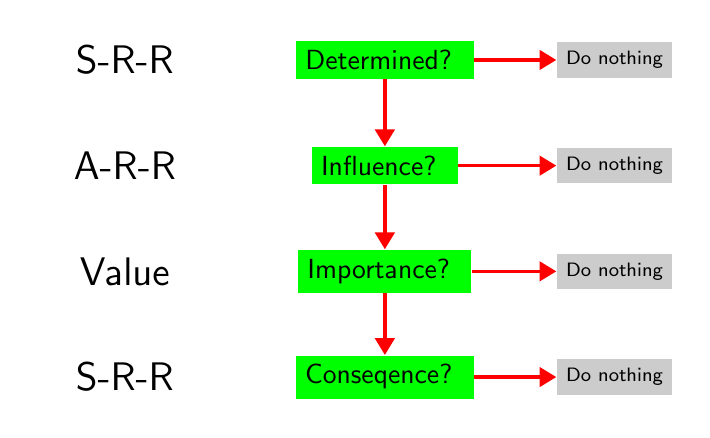
\begin{tikzpicture}
  \matrix (m)
    [
      matrix of nodes,
      column sep      = 3em,
      row sep         = 5ex,
      column 1/.style = { nodes = { empty }  },
      column 2/.style = { nodes = { box }    },
      column 3/.style = { nodes = { result } },
    ]
    {
      S-R-R  & Determined? & \nothing \\
      A-R-R  & Influence?  & \nothing \\
      Value  & Importance? & \nothing \\
      S-R-R  & Conseqence? & \nothing \\
    };
  \foreach \i/\j in {1/2,2/3,3/4} {
    \draw [arrow] (m-\i-2) -- (m-\j-2);
    \draw [arrow] (m-\i-2) -- (m-\i-3);
  }
  \draw [arrow] (m-4-2) -- (m-4-3);
\end{tikzpicture}
\end{document}